\section{Extras}

\subsection{Sorteo de obstáculos}

Aunque no se trate de una mejora en sí del proceso de mapeado, se ha conseguido unir el módulo de sorteo de obstáculos, desarrollado en la primera práctica, junto al módulo implementado. Es por ello que la trayectoria que se muestra en la Figura \ref{fig:clase} resulta tan suave. De esta manera evitamos los saltos bruscos de velocidad y movimiento ocasionados por el módulo de \emph{teleop}.

\subsection{Difuminado}

Sólo por diversión, implementamos un difuminado de la imagen entre las líneas 193 y 198 del fichero \texttt{mapping.cpp}. En la implementación original, el callback \texttt{processOdom} actualiza la variable global \texttt{cv::Mat mymap} coloreando la matriz con datos de tipo \texttt{cv::Vec3b}, es decir, coloreando un píxel en rojo en la posición actual del \emph{turtlebot} y un píxel azul con el obstáculo localizado mediante el lídar. Sin embargo, esta implementación no hace más que ir añadiendo color indefinidamente a la matriz.

Nuestra implementación proponía reducir esos valores de manera constante mientras el escaneado del lídar no volviera a detectar el mismo obstáculo, concretamente, sustrayendo el vector \texttt{cv::Vec3b(12, 0, 1)} a cada elemento de la matriz, lo que supone que aproximadamente en $255 / 12 \approx 21 $ llamadas consecutivas a la función, un píxel que en cierto momento se hubiera detectado como obstáculo (elemento establecido como \texttt{cv::Vec3b(255, 0, 0)} en la matriz), en la llamada 22 desaparecería de la imagen. De manera similar para la trayectoria seguida por el robot, pero esta vez durante 255 llamadas. 

De esta manera, obtenemos un desvanecimiento de imágenes antiguas de forma progresiva, como se observa en la Figura \ref{fig:difuminado}. Se puede apreciar el desvanecimiento de la trayectoria roja, y más sutilmente, los obstáculos azules.

\begin{figure}[!ht]
    \centering
    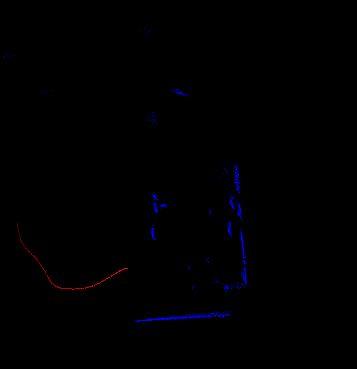
\includegraphics[scale=0.75]{images/difuminado.png}
    \caption{Resultado tras el difuminado aplicado en cada llamada a \texttt{processOdom}.}
    \label{fig:difuminado}
\end{figure}